\documentclass[a4paper,11pt]{article}
\usepackage{amsmath,amsfonts,amssymb,amsthm}
\usepackage{graphicx}
\usepackage{fullpage}
\usepackage{caption}
\usepackage{setspace}
\usepackage{hyperref}
\usepackage{enumerate}
\usepackage[all]{xy}
\usepackage[margin=1in]{geometry}
\usepackage{multirow}
\usepackage{bm}
\usepackage[toc,page]{appendix}
\usepackage{geometry}
\usepackage{siunitx}

\usepackage{listings}
\usepackage{color} %red, green, blue, yellow, cyan, magenta, black, white
\definecolor{mygreen}{RGB}{28,172,0} % color values Red, Green, Blue
\definecolor{mylilas}{RGB}{170,55,241}

\geometry{tmargin=0.7in,bmargin=0.7in,lmargin=0.9in,rmargin=0.9in}

\numberwithin{equation}{section}
\newtheorem{thm}{Theorem}[section]
\newtheorem{lem}[thm]{Lemma}
\newtheorem{cor}[thm]{Corollary}
\newtheorem{exa}[thm]{Example}
\newtheorem{prop}[thm]{Proposition}
\newtheorem{defn}[thm]{Definition}
\newtheorem{claim}[thm]{Claim}
\theoremstyle{remark}
\newtheorem*{rem}{Remark}


\newcommand{\Q}{\mathbb Q}
\newcommand{\Z}{\mathbb Z}
\newcommand{\N}{\mathbb N}
\newcommand{\R}{\mathbb R}
\newcommand{\C}{\mathbb C}
\newcommand{\HH}{\mathbb H}
\newcommand{\F}{\mathbb F}

\DeclareMathOperator*{\argmax}{argmax}


\title{Reinforcement Learning: An Introduction \\ Attempted Solutions \\ Chapter 2}
\author{Scott Brownlie \& Rafael Rui}
\date{}


\begin{document}
%\pagenumbering{gobble}
\maketitle
%\newpage
%\pagenumbering{arabic}

\section{Exercise 2.1}

\textbf{In $\epsilon$-greedy action selection, for the case of two actions and $\epsilon = 0.5$, what is the probability that the greedy action is selected?}
\\ \\
The greedy action is initially selected with probability 0.5, and if not, then one of the two actions is selected randomly (each with probability 0.5). Therefore, the overall probability that the greedy action is selected is
\[
	0.5 + 0.5 \cdot 0.5 = 0.75.
\]


\section{Exercise 2.2: Bandit example}

\textbf{Consider a $k$-armed bandit problem with $k = 4$ actions, denoted 1, 2, 3, and 4. Consider applying to this problem a bandit algorithm using $\epsilon$-greedy action selection, sample-average action-value estimates, and initial estimates of $Q_1(a) = 0$, for all $a$. Suppose the initial sequence of actions and rewards is $A_1 = 1, R_1 = 1, A_2 = 2, R_2 = 1, A_3 = 2, R_3 = 2, A_4 = 2, R_4 = 2, A_5 = 3, R_5 = 0$. On some of these time steps the $\epsilon$ case may have occurred, causing an action to be selected at random. On which time steps did this definitely occur? On which time steps could this possibly have occurred?}
\\ \\
The action value estimates on each time step are as follows:
\begin{enumerate}
	\item $Q_1(1) = 0, Q_1(2) = 0, Q_1(3) = 0, Q_1(4) = 0$
	\item $Q_1(1) = 1, Q_1(2) = 0, Q_1(3) = 0, Q_1(4) = 0$
	\item $Q_1(1) = 1, Q_1(2) = 1, Q_1(3) = 0, Q_1(4) = 0$
	\item $Q_1(1) = 1, Q_1(2) = 3/2, Q_1(3) = 0, Q_1(4) = 0$
	\item $Q_1(1) = 1, Q_1(2) = 5/3, Q_1(3) = 0, Q_1(4) = 0$
	\item $Q_1(1) = 1, Q_1(2) = 5/3, Q_1(3) = 0, Q_1(4) = 0$
\end{enumerate}
The highest actions values on each time step were $\{1,2,3,4\}, \{1\}, \{1, 2\}, \{2\}, \{2\}$ and the chosen actions were $1,2,2,2,3$ respectively.
Therefore, the $\epsilon$ case definitely occurred on time steps 2 and 5. As it is possible that the greedy action is chosen randomly when the $\epsilon$ case occurs, the $\epsilon$ case could possibly have occurred on any of the remaining time steps.


\section{Exercise 2.3}

\textbf{In the comparison shown in Figure 2.2, which method will perform best in the long run in terms of cumulative reward and probability of selecting the best action? How much better will it be? Express your answer quantitatively.}
\\ \\

The $\epsilon=0.01$ case will perform better in the long run. It is guaranteed we will find the optimal action and then exploit it in the long run. Thus, it will exploit the best action  $99\%$ of the time, while the $\epsilon=0.1$  will exploit the optimal action only $90\%$ of the time.
Quantitatively, in the long run the $\epsilon$-greedy strategy will take the wrong action in $1 - \epsilon$. We can compute the asymptotic reward as
 $$(1 - \epsilon) r_{max} + \epsilon r_{mean},$$
where  $r_{mean}$ is the mean reward and  $r_{max}$ is the maximum reward. 

Let's assume that $r_{mean}=0$ (can we assume 0 for a completely random k-armed bandit or use 1 for the suboptimal greedy case????) and $r_{max} =1.5$ (it seems the asymptotic value for $\epsilon$ and also the greater mean value in the Fig 2.1.,  Then, we have 
$$
0.9*1.5 + 0.1 *0 = 1.35 
$$
for $\epsilon=0.1$ and 
$$
0.99*1.5 + 0.01*0 = 1.485
$$
for $\epsilon=0.01$   



\section{Exercise 2.4}

\textbf{If the step-size parameters, $\alpha_n$, are not constant, then the estimate $Q_n$ is a weighted average of previously received rewards with weighting different from that given by (2.6). What is the weighting on each prior reward for the general case, analogous to (2.6), in terms of the sequence of step-size parameters?}
\\ \\ 
We have
\begin{align*}
	Q_{n+1} & = Q_n + \alpha_n[R_n - Q_n] \\
			& = \alpha_n R_n + (1-\alpha_n) Q_n \\
			& = \alpha_n R_n + (1-\alpha_n)[\alpha_{n-1} R_{n-1} + (1-\alpha_{n-1}) Q_{n-1}] \\
			& = \alpha_n R_n + (1-\alpha_n)\alpha_{n-1}R_{n-1} + (1-\alpha_n)(1-\alpha_{n-1})Q_{n-1} \\
			& = \alpha_n R_n + (1-\alpha_n)\alpha_{n-1}R_{n-1} + \quad \dots + (1-\alpha_n)(1-\alpha_{n-1})\dots (1-\alpha_2)\alpha_1 R_1 + \\
			& \quad \quad (1-\alpha_n)(1-\alpha_{n-1})\dots (1-\alpha_2)(1-\alpha_1) Q_1 \\
			& = Q_1\prod_{j=1}^{n}(1-\alpha_j) + \alpha_n R_n + \sum_{i=1}^{n-1}\alpha_i R_i \prod_{j=i+1}^{n}(1-\alpha_j)\\
			& = Q_1\prod_{j=1}^{n}(1-\alpha_j) + \sum_{i=1}^{n}\alpha_i R_i \prod_{j=i}^{n-1}(1-\alpha_{j+1}).
\end{align*}
Therefore, the weighting on $R_n$ is $\alpha_n$ and the weighting on $R_i$ for $i=1,\dots,n-1$ is $\alpha_i \prod_{j=i+1}^{n}(1-\alpha_j)$. Note that when $\alpha_i = \alpha$ for all $i$ the expression above reduces to
\[
	(1-\alpha)^n Q_1 +  \sum_{i=1}^{n-1}\alpha(1-\alpha)^{n-i}R_i = (1-\alpha)^n Q_1 + \sum_{i=1}^{n}\alpha(1-\alpha)^{n-i}R_i,
\]
which is exactly (2.6).


\section{Exercise 2.5}

\textbf{Design and conduct an experiment to demonstrate the difficulties that sample-average methods have for nonstationary problems. Use a modified version of the 10-armed testbed in which all the $q_*(a)$ start out equal and then take independent random walks (say by adding a normally distributed increment with mean zero and standard deviation 0.01 to all the $q_*(a)$ on each step). Prepare plots like Figure 2.2 for an action-value method using sample averages, incrementally computed, and another action-value method using a constant step-size parameter, $\alpha = 0.1$. Use $\epsilon = 0.1$ and longer runs, say of 10,000 steps.}
\\ \\ 
As we can see from Figure \ref{fig:KArmedBanditNonStationarySampleAveraging}, the sample averaging method chooses the optimal action less than 50\% of the time, even after 10,000 time steps. Using a constant step-size of 0.1 works better, as shown in Figure \ref{fig:KArmedBanditNonStationaryConstantStep} where the optimal action is chosen around 75\% of the time after 10,000 time steps.  The sample averaging method does not work as well because after a significant number of time steps the step-size of $1/n$ becomes very small and the action-value estimates cannot adapt to the non-stationary environment.


\begin{figure}
	\centering
	\caption{Average performance of non-stationary $K$-armed bandit with sample averaging.}
	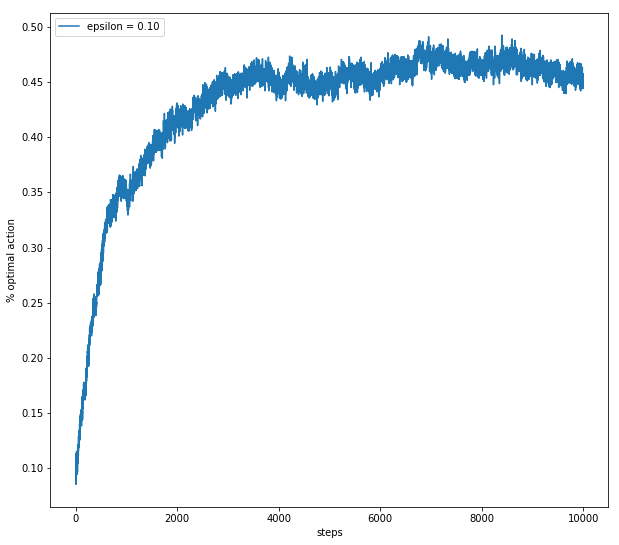
\includegraphics[scale=0.5]{ex2_5_1}
	\label{fig:KArmedBanditNonStationarySampleAveraging}
\end{figure}

\begin{figure}
	\centering
	\caption{Average performance of non-stationary $K$-armed bandit with constant step-size $\alpha=0.1$.}
	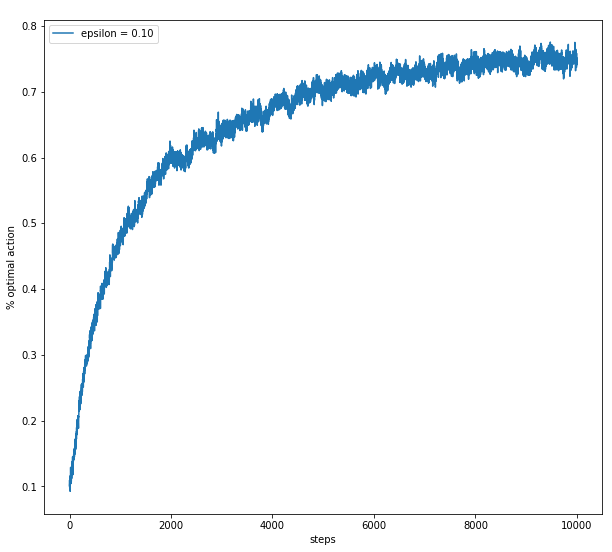
\includegraphics[scale=0.5]{ex2_5_2}
	\label{fig:KArmedBanditNonStationaryConstantStep}
\end{figure}


\section{Exercise 2.6: Mysterious Spikes}

\textbf{The results shown in Figure 2.3 should be quite reliable because they are averages over 2000 individual, randomly chosen 10-armed bandit tasks. Why, then, are there oscillations and spikes in the early part of the curve for the optimistic method? In other words, what might make this method perform particularly better or worse, on average, on particular early steps?}
\\ \\ 
On the 1st time step all arms have an estimated value of 5 and the optimistic method has to choose an action at random. As the $q_*(a)$ are selected from a normal distribution with mean 0 and variance 1, it is extremely unlikely that the reward will be greater than or equal to 5. Therefore, the estimated value of the chosen action will decrease and on the 2nd time step the algorithm will choose randomly between the remaining 9 actions. Again the reward will be less than 5 and the estimated value of this action will decrease and on the 3rd time step the algorithm will choose randomly between the remaining 8 actions. This will continue for the first ten time steps until all ten actions have been selected and their estimated values reduced. Thus, as the selection during the first ten steps is completely random, on each of these steps the optimal value is chosen 10\% of the time on average, as show in the graph.
\\ \\
Now on the 11th time step the action whose value was reduced the least, that is, the action which obtained the greatest reward during the first ten steps, will be selected. Over many runs the optimal action will return the highest reward and will therefore be selected most frequently on the 11th step. From the plot it looks like the first large spike occurs on the 11th step, where the optimal action is selected in just over 40\% of the runs. 
\\ \\
If the optimal action is selected on the 11th step then its estimated value will be reduced further such that it will not realistically be chosen again until after all other actions have also been sampled and had their estimated values reduced. Thus the next realistic opportunity for the optimal action to be selected will be on the 21st step, where there appears to be another spike in the graph up to just under 20\%. If on the other hand the optimal action is not selected on the 11th step then it is the most likely of the remaining nine actions to be selected on the 12th step, and so on. 
\\ \\
After thirty steps each action will likely have been chosen three times and the estimated values will have been reduced such that they are much closer to the true values. As a result, from this point on the spikes in the graph are noticeably smaller.  


\section{Exercise 2.7: Unbiased Constant-Step-Size Trick}

\textbf{In most of this chapter we have used sample averages to estimate action values because sample averages do not produce the initial bias that constant step sizes do (see the analysis leading to (2.6)). However, sample averages are not a completely satisfactory solution because they may perform poorly on nonstationary problems. Is it possible to avoid the bias of constant step sizes while retaining their advantages on nonstationary problems? One way is to use a step size of
\[
	\beta_n \doteq \alpha /  \bar{o}_n,
\]
to process the $n$th reward for a particular action, where $\alpha > 0$ is a conventional constant step size, and $\bar{o}_n$ is a trace of one that starts at 0:
\[
	\bar{o}_n \doteq \bar{o}_{n-1} + \alpha(1-\bar{o}_{n-1}), 	
\]
for $n\geq 0$ with $\bar{o}_0 \doteq 0$. Carry out an analysis like that in (2.6) to show that $Q_n$ is an exponential recency-weighted average \emph{without initial bias}.}
\\ \\ 
We have
\begin{align*}
	Q_{n+1} & = Q_n + \beta_n[R_n - Q_n] \\
	& = \beta_n R_n + (1-\beta_n) Q_n \\
	& = \beta_n R_n + (1-\beta_n)[\beta_{n-1} R_{n-1} + (1-\beta_{n-1}) Q_{n-1}] \\
	& = \beta_n R_n + (1-\beta_n)\beta_{n-1}R_{n-1} + (1-\beta_n)(1-\beta_{n-1})Q_{n-1} \\
	& = \frac{\alpha}{\bar{o}_n} R_n + \left(1-\frac{\alpha}{\bar{o}_n}\right)\frac{\alpha}{\bar{o}_{n-1}}R_{n-1} + \left(1-\frac{\alpha}{\bar{o}_n}\right)\left(1-\frac{\alpha}{\bar{o}_{n-1}}\right)Q_{n-1} \\
	& = \frac{\alpha}{\bar{o}_n} R_n + \left(\frac{\bar{o}_n - \alpha}{\bar{o}_n}\right)\frac{\alpha}{\bar{o}_{n-1}}R_{n-1} + \left(\frac{\bar{o}_n - \alpha}{\bar{o}_n}\right)\left(\frac{\bar{o}_{n-1} - \alpha}{\bar{o}_{n-1}}\right)Q_{n-1} \\
	& = \frac{\alpha}{\bar{o}_n} R_n + \left(\frac{\bar{o}_{n-1} + \alpha(1-\bar{o}_{n-1}) - \alpha}{\bar{o}_n}\right)\frac{\alpha}{\bar{o}_{n-1}}R_{n-1} + \left(\frac{\bar{o}_{n-1} + \alpha(1-\bar{o}_{n-1}) - \alpha}{\bar{o}_n}\right)\left(\frac{\bar{o}_{n-1} - \alpha}{\bar{o}_{n-1}}\right)Q_{n-1} \\
	& = \frac{\alpha}{\bar{o}_n} R_n + \left(\frac{\bar{o}_{n-1}(1 - \alpha)}{\bar{o}_n}\right)\frac{\alpha}{\bar{o}_{n-1}}R_{n-1} + \left(\frac{\bar{o}_{n-1}(1 - \alpha)}{\bar{o}_n}\right)\left(\frac{\bar{o}_{n-1} - \alpha}{\bar{o}_{n-1}}\right)Q_{n-1} \\	
	& = \frac{\alpha}{\bar{o}_n} R_n + \frac{(1-\alpha)\alpha}{\bar{o}_n} R_{n-1} + \frac{(1-\alpha)(\bar{o}_{n-1} - \alpha)}{\bar{o}_n}	Q_{n-1}.		
\end{align*}
Now 
\begin{align*}
	(\bar{o}_{n-1} - \alpha) Q_{n-1} & = (\bar{o}_{n-1} - \alpha) [\beta_{n-2} R_{n-2} + (1-\beta_{n-2}) Q_{n-2}] \\
	& = (\bar{o}_{n-1} - \alpha)\beta_{n-2} R_{n-2} + (\bar{o}_{n-1} - \alpha) (1-\beta_{n-2}) Q_{n-2}	\\
	& = (\bar{o}_{n-1} - \alpha)\frac{\alpha}{\bar{o}_{n-2}} R_{n-2} + (\bar{o}_{n-1} - \alpha)	\left(1-\frac{\alpha}{\bar{o}_{n-2}}\right) Q_{n-2} \\
	& = (\bar{o}_{n-2} + \alpha(1 - \bar{o}_{n-2}) - \alpha)\frac{\alpha}{\bar{o}_{n-2}} R_{n-2} + (\bar{o}_{n-2} + \alpha(1 - \bar{o}_{n-2}) - \alpha)	\left(1-\frac{\alpha}{\bar{o}_{n-2}}\right) Q_{n-2} \\
	& = \bar{o}_{n-2}(1 - \alpha)\frac{\alpha}{\bar{o}_{n-2}} R_{n-2} + \bar{o}_{n-2}(1 - \alpha) \left(\frac{\bar{o}_{n-2} - \alpha}{\bar{o}_{n-2}}\right) Q_{n-2} \\
	& = (1 - \alpha)\alpha R_{n-2} + (1 - \alpha)(\bar{o}_{n-2} - \alpha)  Q_{n-2} \\
\end{align*}
Hence
\begin{align*}
	Q_{n+1} & = \frac{\alpha}{\bar{o}_n} R_n + \frac{(1-\alpha)\alpha}{\bar{o}_n} R_{n-1} + \frac{(1-\alpha)}{\bar{o}_n}[(1 - \alpha)\alpha R_{n-2} + (1 - \alpha)(\bar{o}_{n-2} - \alpha)  Q_{n-2}] \\
	& =  \frac{\alpha}{\bar{o}_n} R_n + \frac{(1-\alpha)\alpha}{\bar{o}_n} R_{n-1} + \frac{(1-\alpha)^2\alpha}{\bar{o}_n} R_{n-2} + \frac{(1-\alpha)^2(\bar{o}_{n-2} - \alpha)}{\bar{o}_n}	Q_{n-2} \\
	& = \frac{\alpha}{\bar{o}_n} R_n + \frac{(1-\alpha)\alpha}{\bar{o}_n} R_{n-1} + \frac{(1-\alpha)^2\alpha}{\bar{o}_n} R_{n-2} + \dots + \frac{(1-\alpha)^{n-1}\alpha}{\bar{o}_n} R_1 + \frac{(1-\alpha)^{n-1}(\bar{o}_1 - \alpha)}{\bar{o}_n}Q_1 \\
	& = \frac{(1-\alpha)^{n-1}(\bar{o}_1 - \alpha)}{\bar{o}_n}Q_1 + \frac{\alpha}{\bar{o}_n} \sum_{i=1}^{n} (1-\alpha)^{n-i} R_i \\
	& = \frac{(1-\alpha)^{n-1}(\bar{o}_0 + \alpha(1 - \bar{o}_0) - \alpha)}{\bar{o}_n}Q_1 + \frac{\alpha}{\bar{o}_n} \sum_{i=1}^{n} (1-\alpha)^{n-i} R_i \\
	& = \frac{(1-\alpha)^{n-1}(\alpha - \alpha)}{\bar{o}_n}Q_1 + \frac{\alpha}{\bar{o}_n} \sum_{i=1}^{n} (1-\alpha)^{n-i} R_i \\
	& = \frac{\alpha}{\bar{o}_n} \sum_{i=1}^{n} (1-\alpha)^{n-i} R_i.
\end{align*}
This shows that $Q_n$ is an exponential recency-weighted average where the weight given to $R_i$ decays exponentially according to the exponent on $1-\alpha$. Also, as the average does not depend on $Q_1$ it has no initial bias.


\section{Exercise 2.8: UCB Spikes}

\textbf{In Figure 2.4 the UCB algorithm shows a distinct spike in performance on the 11th step. Why is this? Note that for your answer to be fully satisfactory it must explain both why the reward increases on the 11th step and why it decreases on the subsequent steps. Hint: If $c = 1$, then the spike is less prominent.}
\\ \\
As an action $a$ is considered a maximizing action when $N_t(a)=0$, during the first 10 steps all 10 actions will be selected in random order, thus the average reward during the first 10 steps is roughly 0 (recall that the $q_*(a)$ are sampled from a normal distribution with mean 0 and standard deviation 1). On the 11th step we have $N_{11}(a)=1$ for all actions $a$, so the action on the 11th step is selected according to $A_{11} = \argmax_a Q_{11}(a)$. Over many runs the greatest $Q_{11}(a)$ will correspond to actions $a$ whose true values are greater than average and the most frequently chosen action will be the optimal action, which is why the reward increases significantly on the 11th step where we see a large spike in the graph.
\\ \\
Now suppose that action $a'$ is chosen on the 11th step. Then on the 12th step we have
\[
	Q_{12}(a') + 2\sqrt{\frac{\ln 12}{2}} \approx 	Q_{12}(a') + 2.23,
\]
whereas for all other actions $a$ we have
\[
Q_{12}(a) + 2\sqrt{\frac{\ln 12}{1}} \approx Q_{12}(a) + 3.15.
\]
Hence, it is extremely unlikely that the action which was chosen on the 11th step will be chosen again on the 12th step, and since the frequency at which an action is chosen on the 11th step is directly proportional to its true value, these same actions will be chosen less on the 12th step, which explains why there is an immediate drop in the average reward.


\section{Exercise 2.9}

\textbf{Show that in the case of two actions, the soft-max distribution is the same as that given by the logistic, or sigmoid, function often used in statistics and artificial neural networks.}
\\ \\
Suppose that we have two actions $a$ and $b$. Then
\begin{align*}
	\Pr\{A_t = a\} & = \frac{e^{H_t(a)}}{e^{H_t(a)} + e^{H_t(b)}} \\
				   & = \frac{1}{1 + e^{H_t(b) - H_t(a)}} \\
				   & = \frac{1}{1 + e^{-(H_t(a) - H_t(b))}},
\end{align*}
and similarly 
\[
	\Pr\{A_t = b\} = \frac{1}{1 + e^{-(H_t(b) - H_t(a))}}.
\]
Define $G_t(a, b) = H_t(a) - H_t(b)$. Then 
\[
	\Pr\{A_t = a\} = \frac{1}{1 + e^{-G_t(a, b)}} = 1 - \frac{1}{1 + e^{G_t(a, b)}}  = 1 - \Pr\{A_t = b\},   
\]
which is the distribution defined by the sigmoid function.


\section{Exercise 2.10}

\textbf{Suppose you face a 2-armed bandit task whose true action values change randomly from time step to time step. Specifically, suppose that, for any time step, the true values of actions 1 and 2 are respectively 0.1 and 0.2 with probability 0.5 (case A) and 0.9 and 0.8 with probability 0.5 (case B). If you are not able to tell which case you face at any step, what is the best expectation of success you can achieve and how should you behave to achieve it? Now suppose that on each step you are told whether you are facing case A or case B (although you still don’t know the true action values). This is an associative search task. What is the best expectation of success you can achieve in this task, and how should you behave to achieve it?}
\\ \\
Suppose we are not able to tell which case we face at any time step. When we choose action 1 the expected reward is
\[
	0.5\cdot 0.1 + 0.5\cdot 0.9 = 0.5.
\]
When we choose action 2 the expected reward is
\[
	0.5\cdot 0.2 + 0.5\cdot 0.8 = 0.5.
\]
Hence, if we are not able to tell which case we face at any time step then the best expected reward we can achieve is 0.5. This can be achieved, for example, by always choosing action 1.
\\ \\
Suppose now that on each time step we are told whether we are facing case A or case B. Assuming that the rewards are deterministic, the first time we are presented with case A we select action 1 and the second time we select action 2. Then we will observe that the value of action 1 is 0.1 and the value of action 2 is 0.2, and from then on we always select action 2 whenever we are presented with case A. We use the same strategy to identify the best action for case B and, after this initial exploration, we always choose action 2 for case A and action 1 for case B, giving an expected reward of
\[
	0.5\cdot 0.2 + 0.5\cdot 0.9 = 0.55.
\]


\section{Exercise 2.11}

\textbf{Make a figure analogous to Figure 2.6 for the nonstationary case outlined in Exercise 2.5. Include the constant-step-size $\epsilon$-greedy algorithm with $\alpha=0.1$. Use runs of 200,000 steps and, as a performance measure for each algorithm and parameter setting, use the average reward over the last 100,000 steps.}
\\ \\
Due to the execution time, we run only for 100,000 steps and the average reward was computed using the last 50,000 steps. 

\begin{figure}
	\centering
	\caption{A parameter study of the various bandit algorithms. Each point is the average reward obtained over 50,000 steps with a particular algorithm at a particular setting of its parameter}
	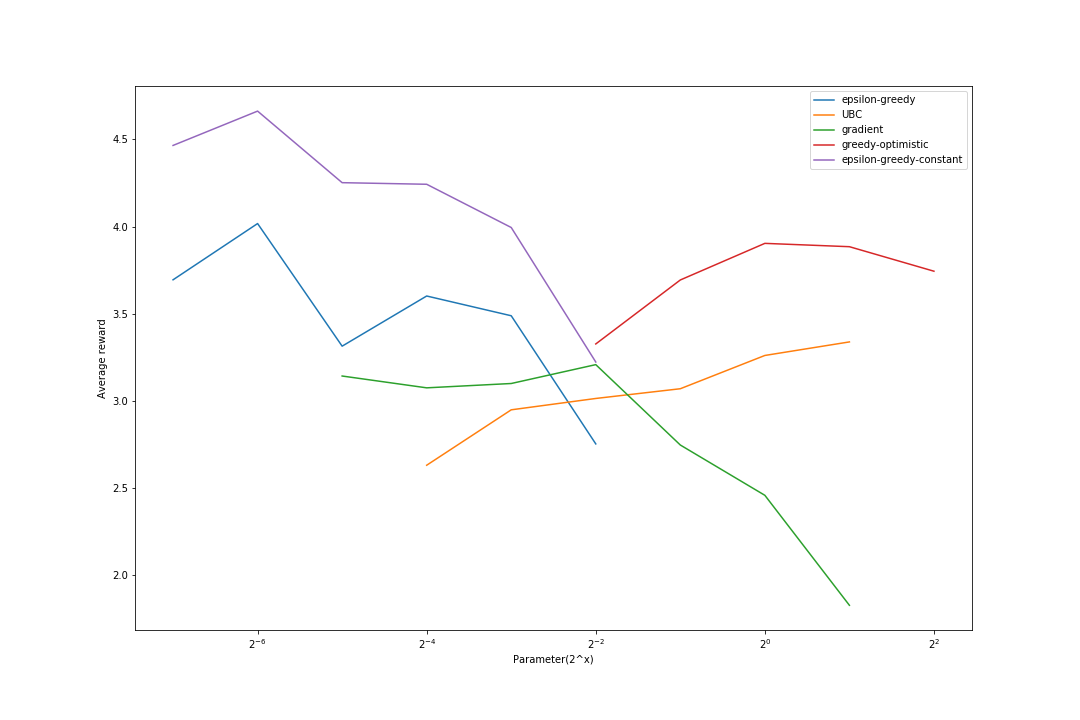
\includegraphics[scale=0.5]{ex2_11}
	\label{fig:KArmedBanditNonStationaryParameterStudy}
\end{figure}


\end{document}